\documentclass[12pt]{article}
\usepackage[utf8]{inputenc}
\usepackage{graphicx}
\usepackage{multicol}
\usepackage{float}
\usepackage{makecell}
\usepackage[a4paper,width=160mm,top=25mm,bottom=25mm]{geometry}

\title{
\vspace{3cm}
\Huge \textbf{Design Document\\}
\vspace{1cm}
\LARGE {COMP208 GROUP PROJECT\\}
\vspace{3cm}
\item
\begin{figure}[H]
\centering
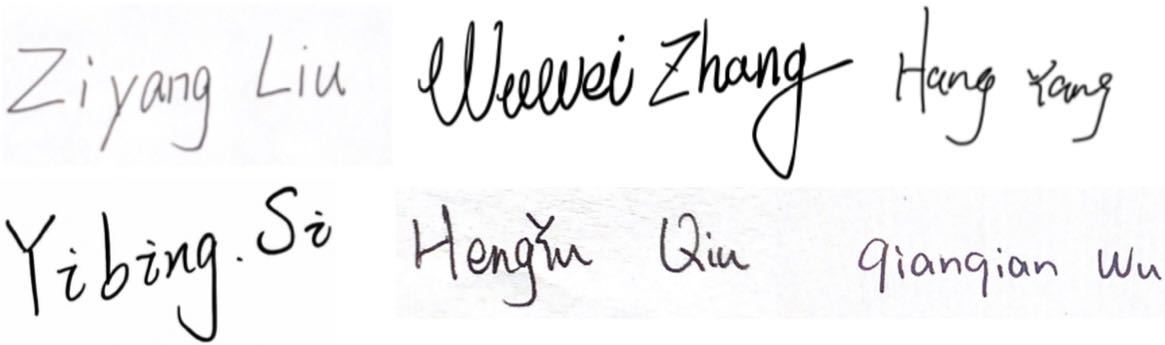
\includegraphics[scale = 0.25]{sign.jpg}
\vspace{2cm}
\end{figure}
}


\author{\LARGE TEAM39\\Ziyang Liu, Wuwei Zhang,Hang Yang, \\Yibing Si, Hengyu Qiu, Qianqian Wu}
\date{March, 2021}

\begin{document}
\maketitle
\newpage
\tableofcontents
\newpage

\section{Changes to Specification}
\subsection{Project Review}
The purpose of our project is to develop a movie website to help users obtain their potential favorite movies based on collaborative filtering which analysis user’s preference and behavior, moreover, to build an interest-oriented platform to record, share ideas and communicate with other users.

\subsection{Changes}
During the design phase of the project, we made three major changes and four supplements based on our initial requirements.\\
First of all, regarding the recommendation algorithm, we decided to use the collaborative filtering algorithm instead of the convolutional neural network. The collaborative filtering algorithm saves time in developing languages, analyzing documents, developing parsing tools and stemming algorithms, mainly focusing on clustering algorithms[1]. On the basis of the Item-based collaborative filtering algorithm, other algorithms may be used to implement process.\\
Second, we decided to use MySQL database instead of other non-relational models. MySQL is a stable and reliable database, and it can be connected to the system to promote the effective management of the database. Its reliability, high performance and on-demand scalability have a significant effect on our data storage and system implementation[2]. We decide to use the TMDb api as the main data source for our website, including movies, actor, genre and cast information. We also use ‘TMDb Dataset’ and ‘The Movies Dataset’ in Kaggle which contains the user’s history and as the data source of the collaborative filtering system.\\
Then, for the choice of front-end and back-end programming, we decided to mainly use HTML, CSS and PHP. And algorithm programming mainly uses Python.\\

\subsection{Supplement}
• Verification of registration - valid email verification is required for registration.\\
• Added Features - Added the ability to view top reviews and actor info pages.\\
• Added user-case - Add user-case such as View actor and Messages notify.\\
• Source Control - Github will be used to do remote cooperation and source control.\\


\section{Database Design}
\subsection{ER Diagram}
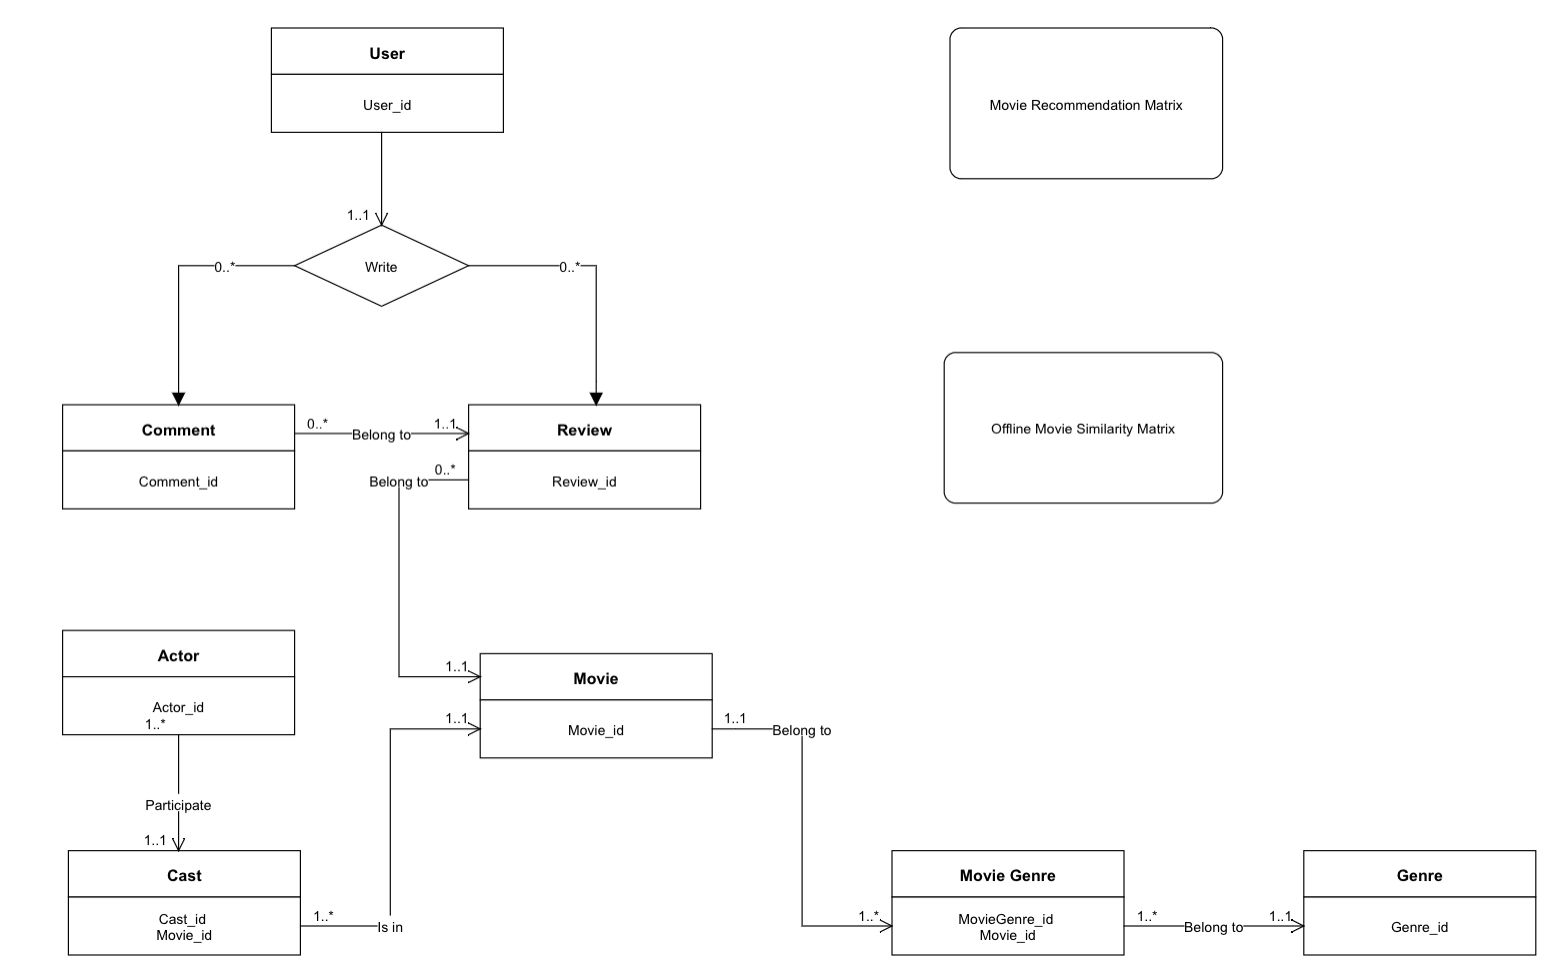
\includegraphics[width=1\linewidth]{ER.jpg}\\
\\The movie will be directly displayed on website based on some filling factor. Each movie belongs to one or many specific genres. Each movie has a particular cast. Each cast consists of one or many actors. Each review is published by one particular user. And each comment is under one particular review, each comment is published by one particular user. Once visitor completing register, he or she will become a user. Movie genre is the implied relation between movie and genre.\\
Offline movie similarity matrix is derived through recommend system, the Collaborative filters will generate save a cosine similarity matrix to check the similarity between movies.\\
Movie recommendation matrix is derived through recommend system, the Collaborative filters will constantly save and modify this matrix based on the user's ranking and the features of movies then put the (movie\_id,recommend level) tuple with higher score to the front position of the list.\\
\newpage

\subsection{Data Dictionary}
In this section, there are 4 types of dictionary. The first is an entities table. This table formulate the name of each entity and explain the occurrence of each. Second is the table of each attribute of entities. We stipulate the data type, length, and key of attributes, and for each attribute we determine whether it can be null or multi-valued or not. The third table is the relation table, it describes the relation type, name between entities. The last is a derivative table. It contains the important derivative data and its structure in the collaborative filtering part.\\

\begin{table}[H]
\centering
\renewcommand\arraystretch{1.08}
\caption{Entities Table}
	\begin{tabular}{|l l l l|}
	    \hline
	    Entity Name &Description&	Aliases &Occurrence\\
        \hline
        Movie&
        \makecell[l]{The movie itself, \\the major content \\in our website}
        &Film
        &\makecell[l]{Will be directly displayed\\ on website based on\\ some filling factor}\\
        \hline
        MovieGenre
        &\makecell[l]{The movie with \\one of its genres}
        &\makecell[l]{}
        &\makecell[l]{The implied relation \\between movie and genre
}\\
        \hline
        Genre
        &\makecell[l]{The type of \\the movie}
        &\makecell[l]{type, style, label}
        &\makecell[l]{Each movie belongs to 1\\or many specific genres}\\
        \hline
        Cast
        &\makecell[l]{The movie \\participants}
        &\makecell[l]{members, participants}
        &\makecell[l]{Each movie has \\a particular cast}\\
        \hline
        Actor
        &\makecell[l]{The director \\or performer}
        &\makecell[l]{Director, Actor, \\Performer, Actress}
        &\makecell[l]{Each cast consists of \\one or many actors }\\
        \hline
        Review
        &\makecell[l]{The review and \\ranking from user}
        &\makecell[l]{score, grade, \\evaluation}
        &\makecell[l]{Each review is published \\by one particular user}\\
        \hline
        Comment
        &\makecell[l]{The comment under \\the review}
        &\makecell[l]{}
        &\makecell[l]{Each comment is under a\\ particular review, each \\comment is published by \\one particular user}\\
        \hline
       User
        &\makecell[l]{ The people who has \\registered in our \\website}
        &\makecell[l]{}
        &\makecell[l]{Once visitor completing\\ register, he/she becomes\\ a user
}\\  
        \hline
	\end{tabular}
\end{table}


\begin{table}[H]
\centering
\renewcommand\arraystretch{1.08}
\caption{Attributes Table}
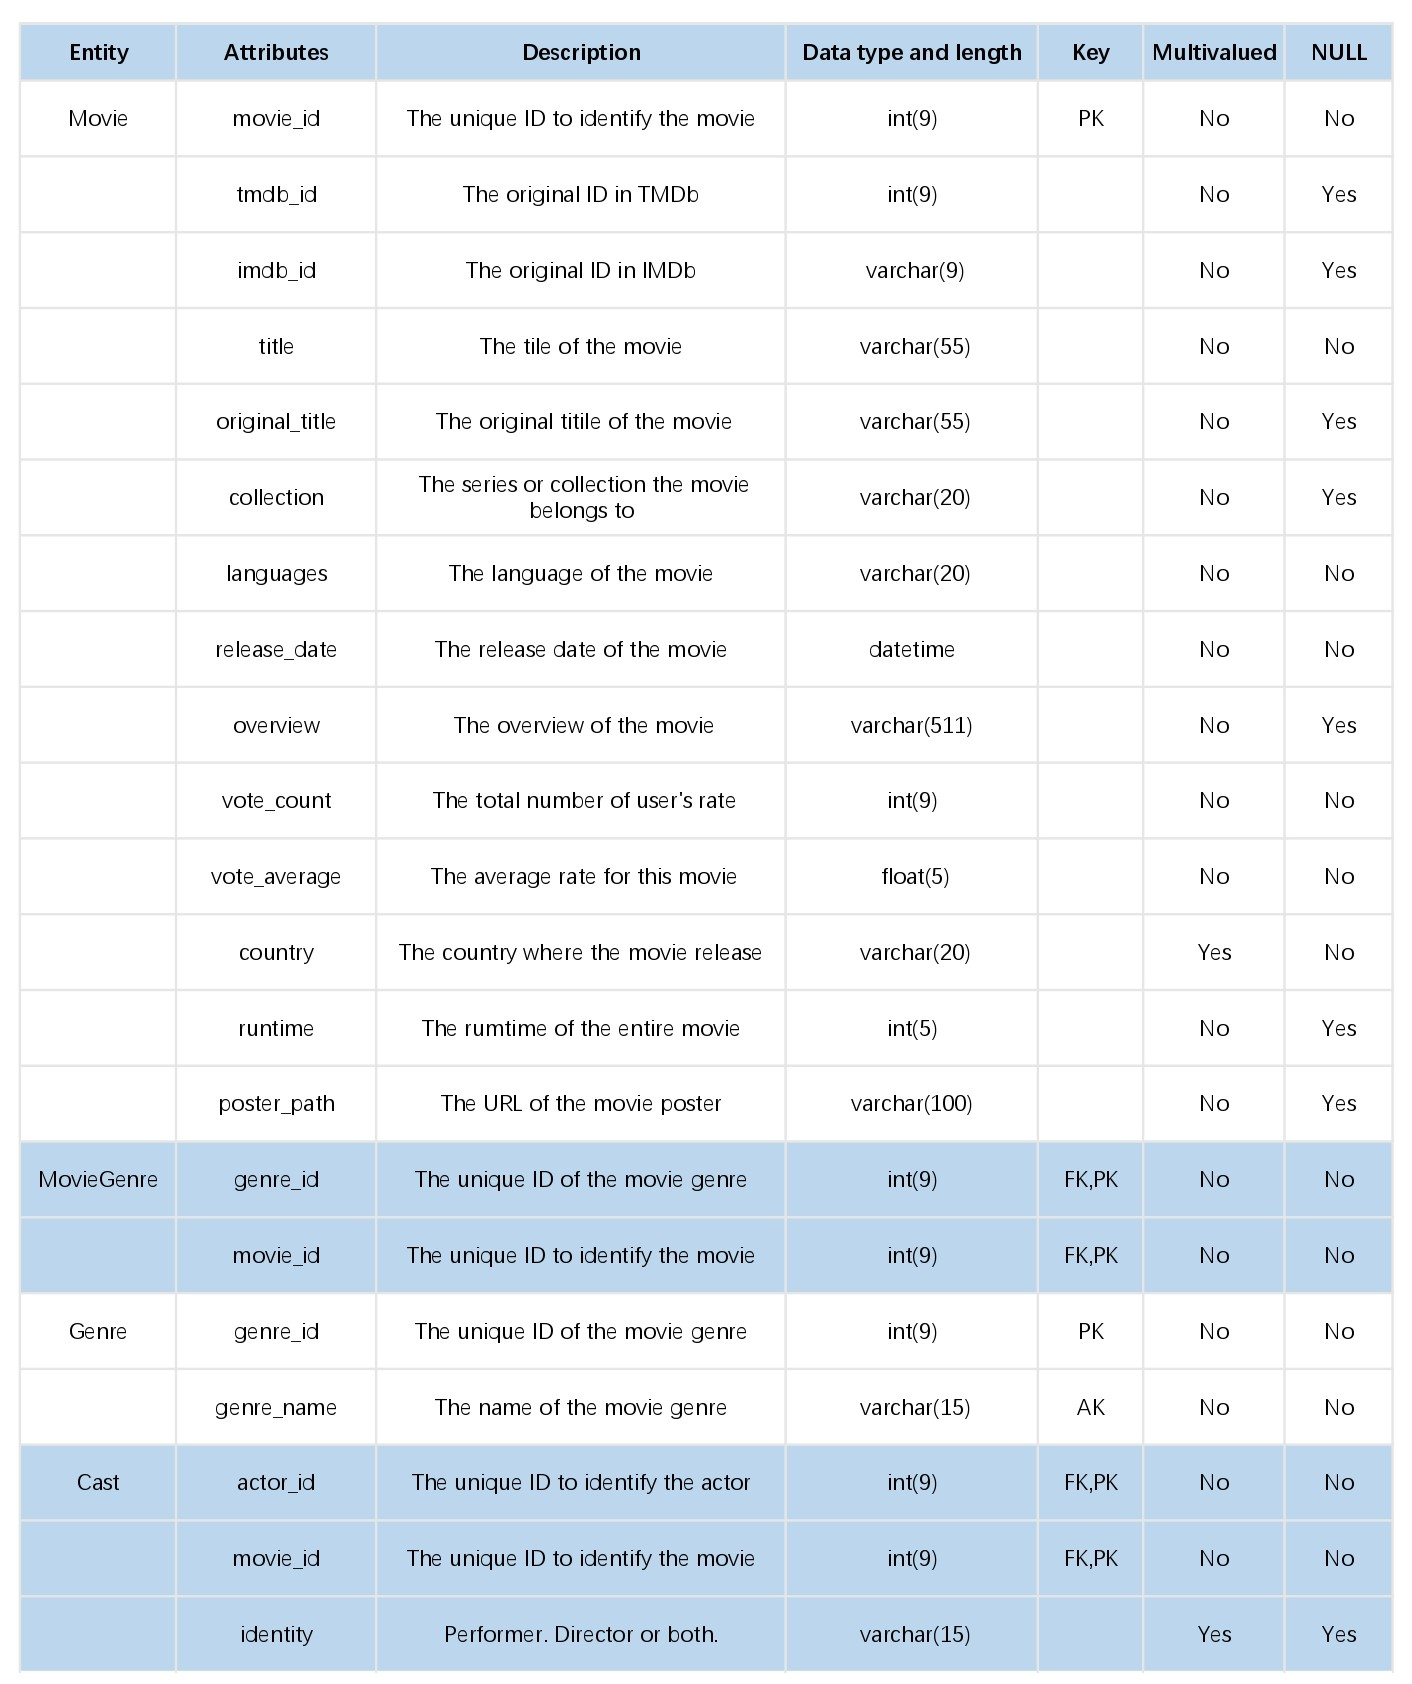
\includegraphics[width=1\linewidth]{a1.jpg}
\end{table}
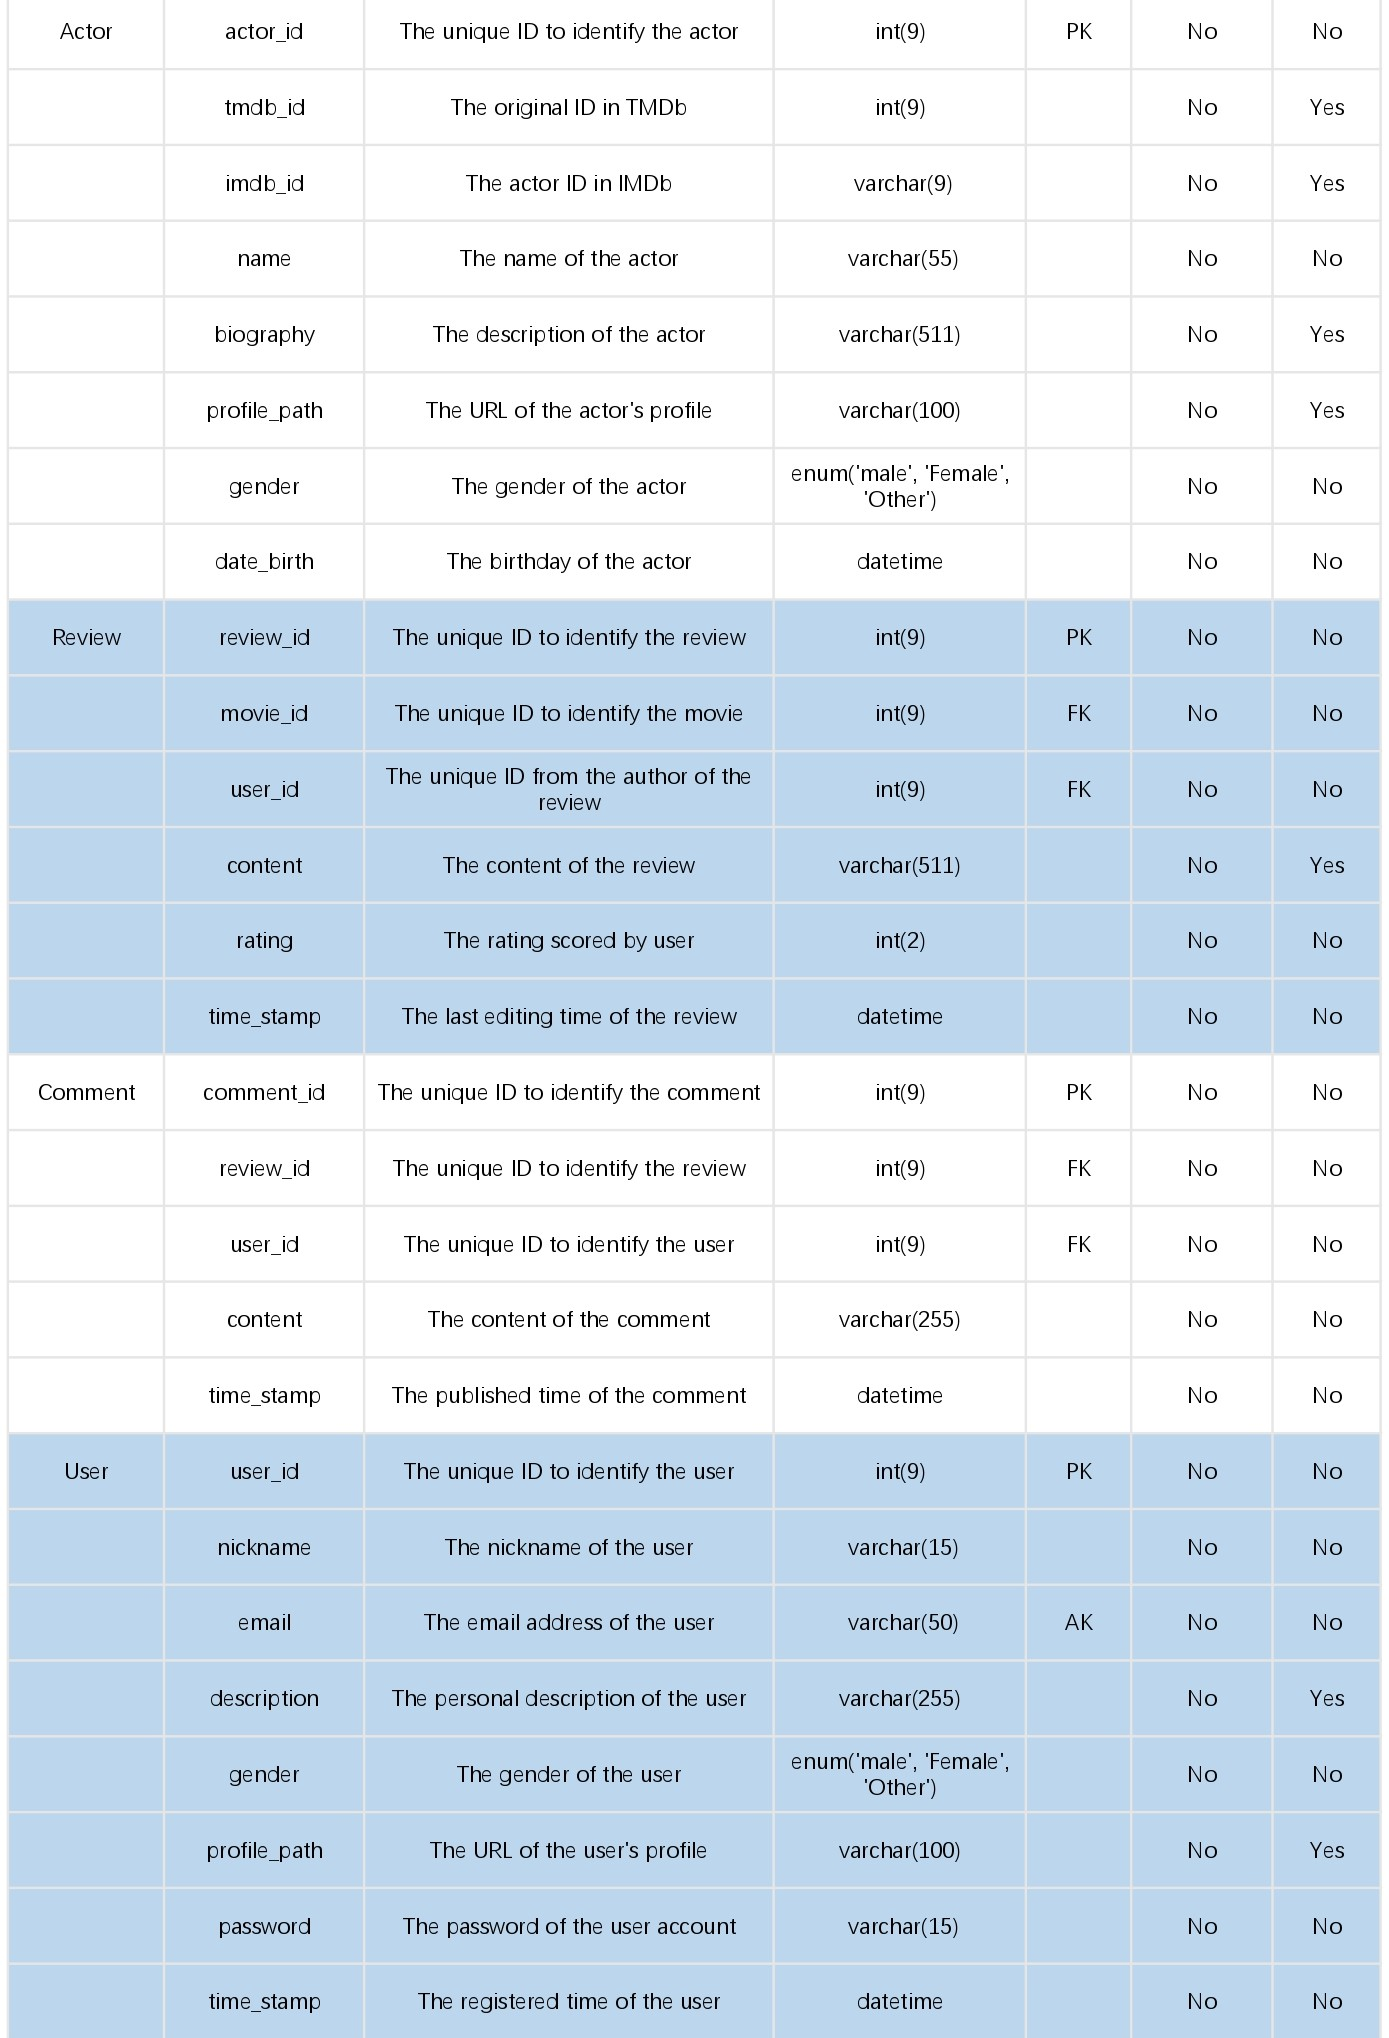
\includegraphics[width=1\linewidth]{a2.jpg}

\begin{table}[H]
\centering
\renewcommand\arraystretch{1.08}
\caption{Relation Table}
	\begin{tabular}{|l l l l l|}
	    \hline
	    Entity name & Description& Aliases & Occurrence &Entity\\
        \hline
        Movie&	 1...1&	 has&	 0...*&	Review\\
        Movie&	 1...1&	has&	 1...*&	Cast\\
        Movie&	 1...1&	belong to&	 1...*&	MovieGenre\\
        MovieGenre&	 1...*&	has& 1...1&	Movie\\
        MovieGenre&	 1...*&	belong to&	 1...1&	Genre\\
        Genre&	 1...1&	has& 1...*&	MovieGenre\\
        Cast&	1...*&	belong to& 	1…1	&Movie\\
        Cast&	 1...1&	has&	 1...*&	Actor\\
        Actor&	1...*&	participate&	 1...1&	Cast\\
        Review&	 1...*&	is in&	 1...1&	Movie\\
        Review&	 1...1&	has&	 0...*&	Comment\\
        Review&	 0...*&	is witten by&	 1...1&	User\\
        Comment&	 0...*&	belong to&	 1...1&	Review\\
        Comment& 0...*&	is witten by&	 1...1&	User\\
        User&	 1...1&	write&	 0...*&	Review\\
        User&	 1...1&	write&	 0...*&	Comment\\
        \hline
	\end{tabular}
\end{table}

\begin{table}[H]
\centering
\renewcommand\arraystretch{1.08}
\caption{Derivative Matrix}
	\begin{tabular}{|l l l|}
	    \hline
	    matrix\_name&head(row(x))&tail(row(x))\\
        \hline
        *offline movie similarity matrix&movie\_id (int)	&list[(movie\_id, similarity)]\\
		\hline
		*movie recommendation matrix&user\_id (int)&list[(movie\_id, recommend level)]\\
		\hline
	\end{tabular}
		\begin{tabular}{l}
		\\
	    \makecell[l]{*Offline movie similarity matrix stores the similarity between movies \\Each row is a list within specific limited length, the similarity is sorted\\ in Descending order. The head of the row is the movie\_id, the tail is the\\list of tuples for (movie\_id. similarities)}
	    \\\\
	    \makecell[l]{*Movie recommendation matrix stores the recommended movie for users.\\ Each row is a list within specific limited length, the recommend level is \\sorted in Descending order. the head of the row is the movie\_id, the tail \\lis theist of tuples for (movie\_id. recommend level)}\\
	\end{tabular}
\end{table}

		
\subsection{Logical Table Structure}

\begin{table}[H]
\centering
\renewcommand\arraystretch{1.08}
	\begin{tabular}{|l|}
		\hline
		\textbf{Movie} (movie\_id, tmdb\_id, imdb\_id, title, original\_title, collection, languages\\release\_date overview, vote\_count, vote\_average, country, runtime, poster\_path)\\
		\textbf{Primary Key} movie\_id\\
        \hline
        \textbf{MovieGenre} (genre\_id, movie\_id)\\
        \textbf{Primary Key} movie\_id\\
        \textbf{Primary Key} genre\_id\\
        \textbf{Foreign Key} movie\_id \textbf{References} Movie(movie\_id)\\
        \textbf{Foreign Key} genre\_id \textbf{References} Genre(genre\_id)\\
        \hline
        \textbf {Genre}(genre\_id, genre\_name)\\
        \textbf{Primary Key} genre\_id\\
        \textbf{Alternate Key} genre\_name\\
        \hline
        \textbf{Cast} (actor\_id, movie\_id, identity)\\
        \textbf{Primary Key} actor\_id\\
        \textbf{Primary Key} movie\_id\\
        \textbf{Foreign Key} actor\_id \textbf{References} Actor(actor\_id)\\
        \textbf{Foreign Key} movie\_id \textbf{References} Movie(movie\_id)\\
        \hline
        \textbf {Actor}(actor\_id, tmdb\_id, imdb\_id, name, biography, profile\_path, gender, date\_birth)\\
        \textbf{Primary Key} actor\_id\\
        \hline
        \textbf{Review} (review\_id, movie\_id, user\_id, content, rating, time\_stamp)\\
        \textbf{Primary Key} review\_id\\
        \textbf{Foreign Key} user\_id \textbf{References} User(user\_id)\\
        \textbf{Foreign Key} movie\_id \textbf{References} Movie(movie\_id)\\ \hline
        \textbf{Comment} (comment\_id, review\_id, user\_id, content, time\_stamp)\\
        \textbf{Primary Key} comment\_id\\
        \textbf{Foreign Key} user\_id \textbf{References} User(user\_id)\\
        \textbf{Foreign Key} review\_id \textbf{References} Review(review\_id)\\
        \hline
        \textbf {User}(user\_id, nickname, email, description, gender ,profile\_path, password, time\_stamp)\\
        \textbf{Primary Key} user\_id\\
        \textbf{Alternate Key} email\\
        \hline
	\end{tabular}
\end{table}
The logical table is the expansion of the ER Diagram.
As the diagram shows, the relation between Movie and Review, Cast, MovieGenre is all 1:m, therefore we use movie\_id in Review, Cast, MovieGenre as the FK because the movie\_id is the PK of the Movie. Moreover, as the Cast, MovieGenre is the derivative relation between movie and actor, genre. We also use actor\_id as the FK in Cast, genre\_id as the FK in MovieGenre. Therefore, the PK in Cast is (actor\_id, movie\_id), the PK in MovieGenre is (genre\_id, movie\_id).
The one user can write many Review and Comment, therefore the user\_id us the FK in Review and Comment. One Comment belongs to one Review but one Review can have many Comment, therefore the review\_id is the FK in comment. One movie can have many review, thus the movie\_id in Review can be used to identify that movie the Review belongs to.\\

\subsection{Physical Table Structure}

\begin{table}[H]
\centering
\renewcommand\arraystretch{1.12}
	\begin{tabular}{l l l l}
		\hline
		&Domain & ID & integer with fixed length 9\\
		&Domain & Imdb & fixed char with length 9\\
        &Domain & Title & varchar with max length 55\\
        &Domain & Date  & fixed length of char format yyyy-mm-dd\\
        &Domain & Details & varchar with max length 20\\
        &Domain & Overview & varchar with max length 511\\
        &Domain & Vote\_count & variable length integer with max length 9\\
        &Domain & Vote\_average & float between 1-10 and with precision 5\\
        &Domain & Run\_time  & variable length integer with max length\\
        &Domain & File\_path & varchar with max length 100\\&&&
        \\Movie(&movie\_id&ID&NOT NULL,\\
        &tmbd\_id&ID&,\\
        &imbd\_id&Imbd&,\\
        &title&Title&NOT NULL,\\
        &original\_title&Title&,\\
        &collection&Details&,\\
        &languages&Details&NOT NULL,\\
        &release\_date&Date&NOT NULL,\\
        &overview&Overview&,\\
        &vote\_count&Vote\_count&NOT NULL,\\
        &vote\_average&Vote\_average&NOT NULL,\\
        &country&Details&NOT NULL,\\
        &runtime&Run\_time&,\\
        &poster\_path&File\_path&  \hspace{4PT} )\\
        &\textbf{Primary Key}& movie\_id&\\
		\hline 
		&Domain & ID & integer with fixed length 9\\&&&
        \\MovieGenre(&movie\_id&ID&NOT NULL,\\& genre\_id&ID&NOT NULL \hspace{4PT} )\\
        &\textbf{Primary Key}& movie\_id&\\
        &\textbf{Primary Key}& genre\_id&\\
        &\textbf{Foreign Key}& movie\_id &\textbf{References} Movie(movie\_id)\\
        &\textbf{Foreign Key}& genre\_id&\textbf{References} Genre(genre\_id)\\
        
		\hline
		&Domain & ID & integer with fixed length 9\\
		&Domain & Name & varchar with max length 15\\&&&
        \\Genre(& genre\_id&ID&NOT NULL,
        \\&genre\_name&Name&NOT NULL\hspace{4PT} )\\
        &\textbf{Primary Key}& genre\_id&\\
        &\textbf{Alternate Key}& genre\_name&\\
        \hline
	\end{tabular}
\end{table}


\begin{table}[H]
\renewcommand\arraystretch{1.1}
\centering

	\begin{tabular}{l l l l}
        \hline
        &Domain & ID & integer with fixed length 9\\
		&Domain & Name & varchar with max length 15\\
        \\Cast(
        & movie\_id & ID & NOT NULL,\\
        & actor\_id & ID & NOT NULL,\\
        & identity & Name &\hspace{4PT} )\\
        &\textbf{Primary Key}& movie\_id&\\
        &\textbf{Primary Key}& actor\_id&\\
        &\textbf{Foreign Key}& movie\_id &\textbf{References} Movie(movie\_id)\\
        &\textbf{Foreign Key}& actor\_id&\textbf{References} Actor(actor\_id)\\
        \hline
        &Domain & ID & integer with fixed length 9\\
		&Domain & Imdb & fixed char with length 9\\
		&Domain & Name & varchar with max length 55\\
		&Domain & Date  & fixed length of char format yyyy-mm-dd\\
        &Domain & Biography & varchar with max length 511\\
        &Domain & File\_path	& varchar with max length 100\\
        &Domain & Gender & enumeration char of ('male', 'Female', 'Other')\\&&&
        \\Actor(& actor\_id&ID&NOT NULL,
        \\&tmdb\_id&ID&,
        \\&Imdb\_id&Imdb&,
        \\&name&Name&NOT NULL,
        \\&biography&Biography&,
        \\&profile\_path&File\_path&,
        \\&gender&Gender&NOT NULL,
        \\&date\_birth&Date&NOT NULL
        \hspace{4PT} )\\
        &\textbf{Primary Key}& actor\_id&\\
		\hline
		&Domain & ID & integer with fixed length 9\\
		&Domain & Imdb & fixed char with length 9\\
		&Domain & Name & varchar with max length 55\\
		&Domain & Date  & fixed length of char format yyyy-mm-dd\\
        &Domain & Biography & varchar with max length 511\\
        &Domain & File\_path	& varchar with max length 100\\
        &Domain & Gender & enumeration char of ('male', 'Female', 'Other')\\&&&
        \\Actor(& actor\_id&ID&NOT NULL,
        \\&tmdb\_id&ID&,
        \\&imdb\_id&Imdb&,
        \\&name&Name&NOT NULL,
        \\&biography&Biography&,
        \\&profile\_path&File\_path&,
        \\&gender&Gender&NOT NULL,
        \\&date\_birth&Date&NOT NULL
        \hspace{4PT} )\\
        &\textbf{Primary Key}& actor\_id&\\
        \hline
	\end{tabular}
\end{table}



\begin{table}[H]
\renewcommand\arraystretch{1.1}
\centering
	\begin{tabular}{l l l l}
		\hline
		&Domain & ID & integer with fixed length 9\\
		&Domain & Time  & char format yyyy-mm-dd hh:mm:ss\\
        &Domain & Content & varchar with max length 511\\
        &Domain & Rating & int between 1-10\\
        
        \\Review(
        & review\_id & ID & NOT NULL,\\
        & movie\_id & ID & NOT NULL,\\
        & user\_id & ID & NOT NULL,\\
        & content & Content &,\\
        & rating & Rating & NOT NULL,\\
        & time\_stamp & Time & NOT NULL
        \hspace{4PT} )\\
        &\textbf{Primary Key}& review\_id&\\
        &\textbf{Foreign Key}& movie\_id &\textbf{References} Movie(movie\_id)\\
        &\textbf{Foreign Key}& user\_id&\textbf{References} User(user\_id)\\
		\hline
		&Domain & ID & integer with fixed length 9\\
		&Domain & Time  & char format yyyy-mm-dd hh:mm:ss\\
        &Domain & Content & varchar with max length 255\\
        
        \\Comment(
        & comment\_id & ID & NOT NULL,\\
        & review\_id & ID & NOT NULL,\\
        & user\_id & ID & NOT NULL,\\
        & content & Content &,\\
        & time\_stamp & Time & NOT NULL
        \hspace{4PT} )\\
        &\textbf{Primary Key}& comment\_id&\\
        &\textbf{Foreign Key}& review\_id &\textbf{References} Review(review\_id)\\
        &\textbf{Foreign Key}& user\_id&\textbf{References} User(user\_id)\\
		\hline
		&Domain & ID & integer with fixed length 9\\
		&Domain & Name & varchar with max length 15\\
		&Domain & Email & varchar with max length 50\\
		&Domain & Description & varchar with max length 255\\
        &Domain & Gender & enumeration ('male', 'Female', 'Other')\\
        &Domain & File\_path& varchar with max length 100\\
        &Domain & Password & varchar with min length 9 max length 15\\
        &Domain & Time  & char format yyyy-mm-dd hh:mm:ss\\

        \\User(& user\_id&ID&Password
        \\&nickname&Name&NOT NULL,
        \\&email&Email& NOT NULL,
        \\&description&Description&,
        \\&gender&Gender&NOT NULL,
        \\&profile\_path&File\_path&,
        \\&password&Password&NOT NULL,
        \\& time\_stamp & Time & NOT NULL
        \hspace{4PT} )\\
        &\textbf{Primary Key}& user\_id&\\
        &\textbf{Alternate Key}& email&\\
        \hline
	\end{tabular}
\end{table}\newpage

\section{Business Rules}
\subsection{Business Polices}
\textbf{-}	Once visitor completing register, he/she becomes a user.\\
\textbf{-}	Only registered users may use comment and review.\\
\textbf{-}	Users have the right to score movies.\\
\textbf{-}	The web may recommend few movies to users.\\
\textbf{-}	Every movie will be classified\\

\subsection{Business Rules}
\textbf{-}	Each user should set up to 9 account ID and 15 digits password.\\
\textbf{-}	Each movie belongs to one or many specific genres.\\
\textbf{-}  Each user can only be recommended at most 50 movies at one time.\\
\textbf{-}  Each Email Address can only be used to register one account.\\

\subsection{Business Rules force constraints on the data in the database}
\textbf{-}  The email under different user\_id must be unique.\\
\textbf{-}	Each movie in the database will be related to one or different genres.\\
\textbf{-}	The user’s account ID is limited to 9 digit and the password is limited to 9-15 characters.\\
\textbf{-}	Each comment is under one particular review, each comment is published by one particular use.\\

\subsection{Privacy Policy and Terms of Service}
This website formulates privacy policies and related clauses to protect the interests of users.\\
The main purpose is to demonstrate how the system collects user data and what services the system will provide:\\
1. Register as a user\\
To complete the creation of an account, you need to provide an email address for verification of registration. After the user registration is completed, your email address will be used as the log in account name by default. If you do not agree, you will not be able to complete the registration.\\
The above information you provide will continue to authorize us to use it during your use of this service. When you delete your account, we will stop using and delete the above information.\\
2. Message notification\\
Message notifications are set up on the website to facilitate you to receive daily movie recommendations, reminders on new movies, and user comment responses in time.\\
More importantly, the website should not provide third-party organizations with any function to sell user information.\\

\subsection{Validation Rules}
1. If a user is not registered and wants to access the system (such as the homepage), then the server will detect whether there is a record of the user in the session. If not, then this user will be restricted by permission and cannot view comments, because only if the user inputs the correct email and password, would the server record their ids in the session. \\
2. Regular expression can be used to check users’ password. Finally, the most of cases that the server recognizes users is to specify their ids in the URL, which is a kind of GET method of HTTP request. \\
3. When a user wants to post a comment, the server will first check whether the current sender is the user recorded in the conversation, and check whether the recipient does exist in the database. \\ 

\section{Transaction Table/Matrix}
\textbf{I: Insert R: Read U: Update D: Delete}\\\\
Transactions:\\ 
a)	Create movie profile\\
b)	Edit genre \\
c)	Create User\\
d)	Create Actor\\
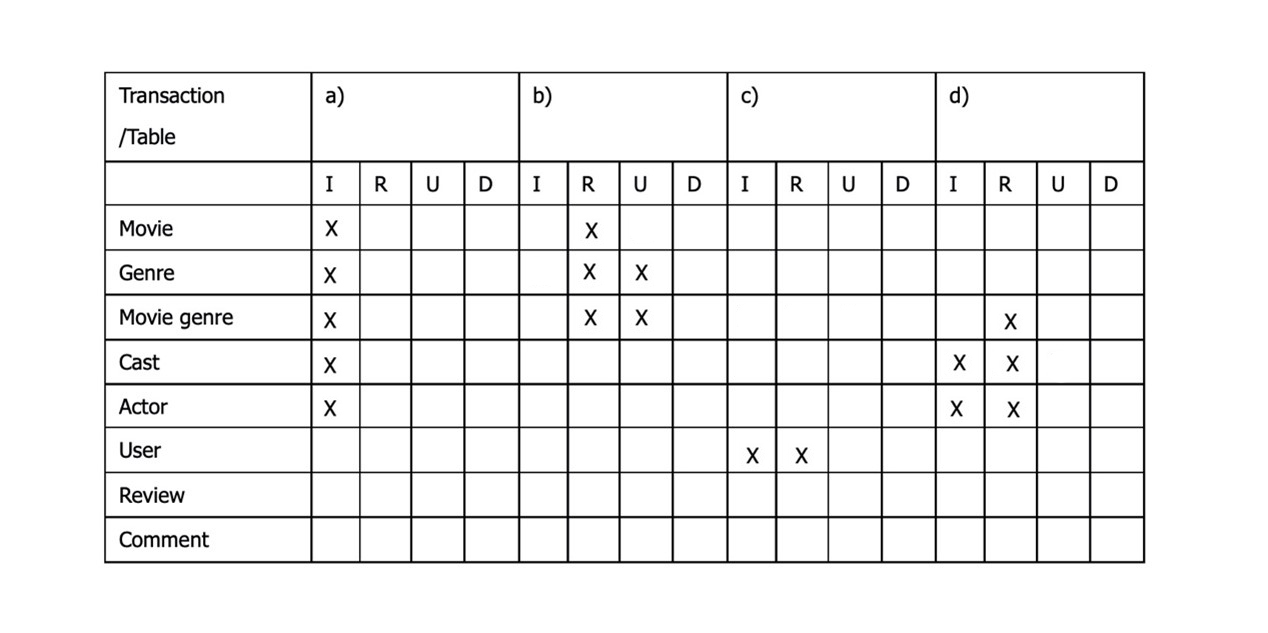
\includegraphics[width=1\linewidth]{tm1.jpg}
\\
Transactions:\\
e)	Edit actor \\
f)	Create review\\
g)	Create comment\\
h)	Delete movie\\
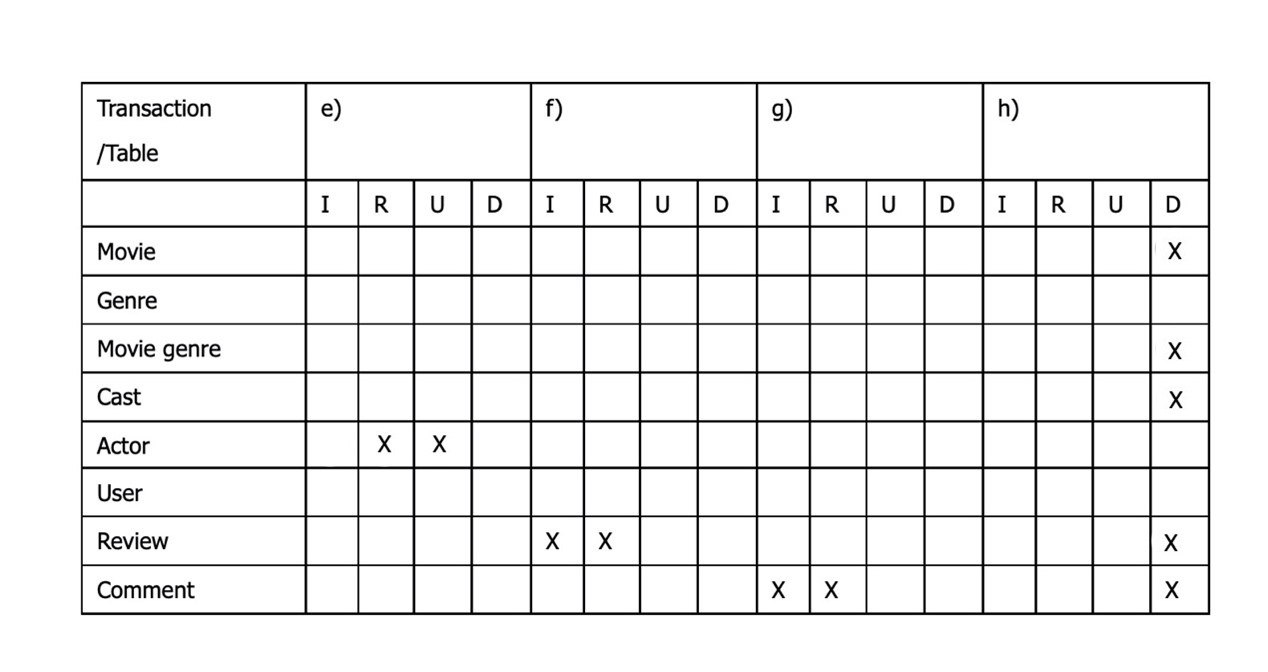
\includegraphics[width=1\linewidth]{tm2.jpg}
\\
Transactions:\\
i)	Delete user\\
j)	Edit cast \\
k)	Delete comment\\
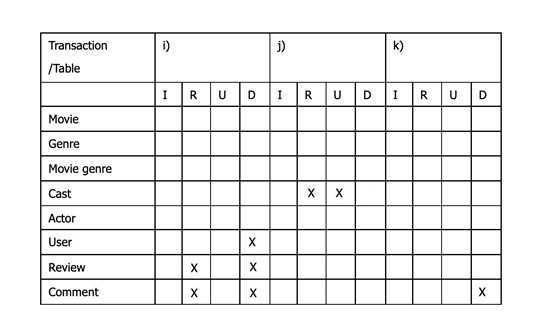
\includegraphics[width=1\linewidth]{tm3.jpg}
\newpage
\section{Algorithm Design}
The key algorithm is Item-based and User-based collaborative filtering algorithm. Item-based collaborative filtering algorithm recommends movies that are similar to the movies users liked before. That means to find the relevance of movies based on the user's historical information, and then generate recommendation information.\\
The steps of this algorithm are to first calculate the similarity between the movies, and then calculate the predicted value to predict and recommend the movies that the user has not scored.\\
The advantage of this algorithm is that it has strong interpret-ability and meets real-time requirement, so we use it to recommend movies that users might like.\\
Below is a simple picture description of this algorithm:\\
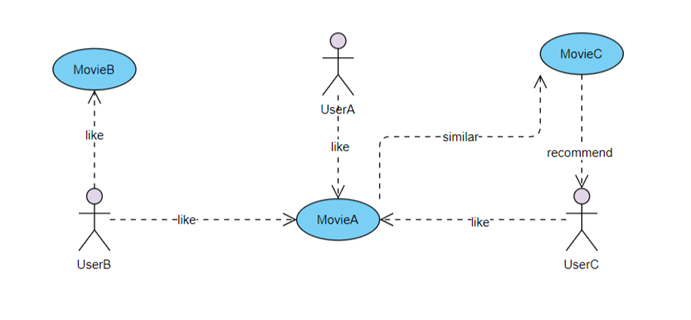
\includegraphics[width=1\linewidth]{alg.png}\\
The recommendation system also uses the user-based collaborative filtering algorithm, which can recommends movies that other users with similar interests like, so it is used to recommend movies with high popularity to the user.\\
The user-based collaborative filtering algorithm mainly includes two steps. The first is to find the collection of users with similar interests to the target user. Then find movies in this collection that users like and that the target user has not heard of and recommend them to the target user.\\

\section{Process Design}
\subsection{Use Case Diagram}
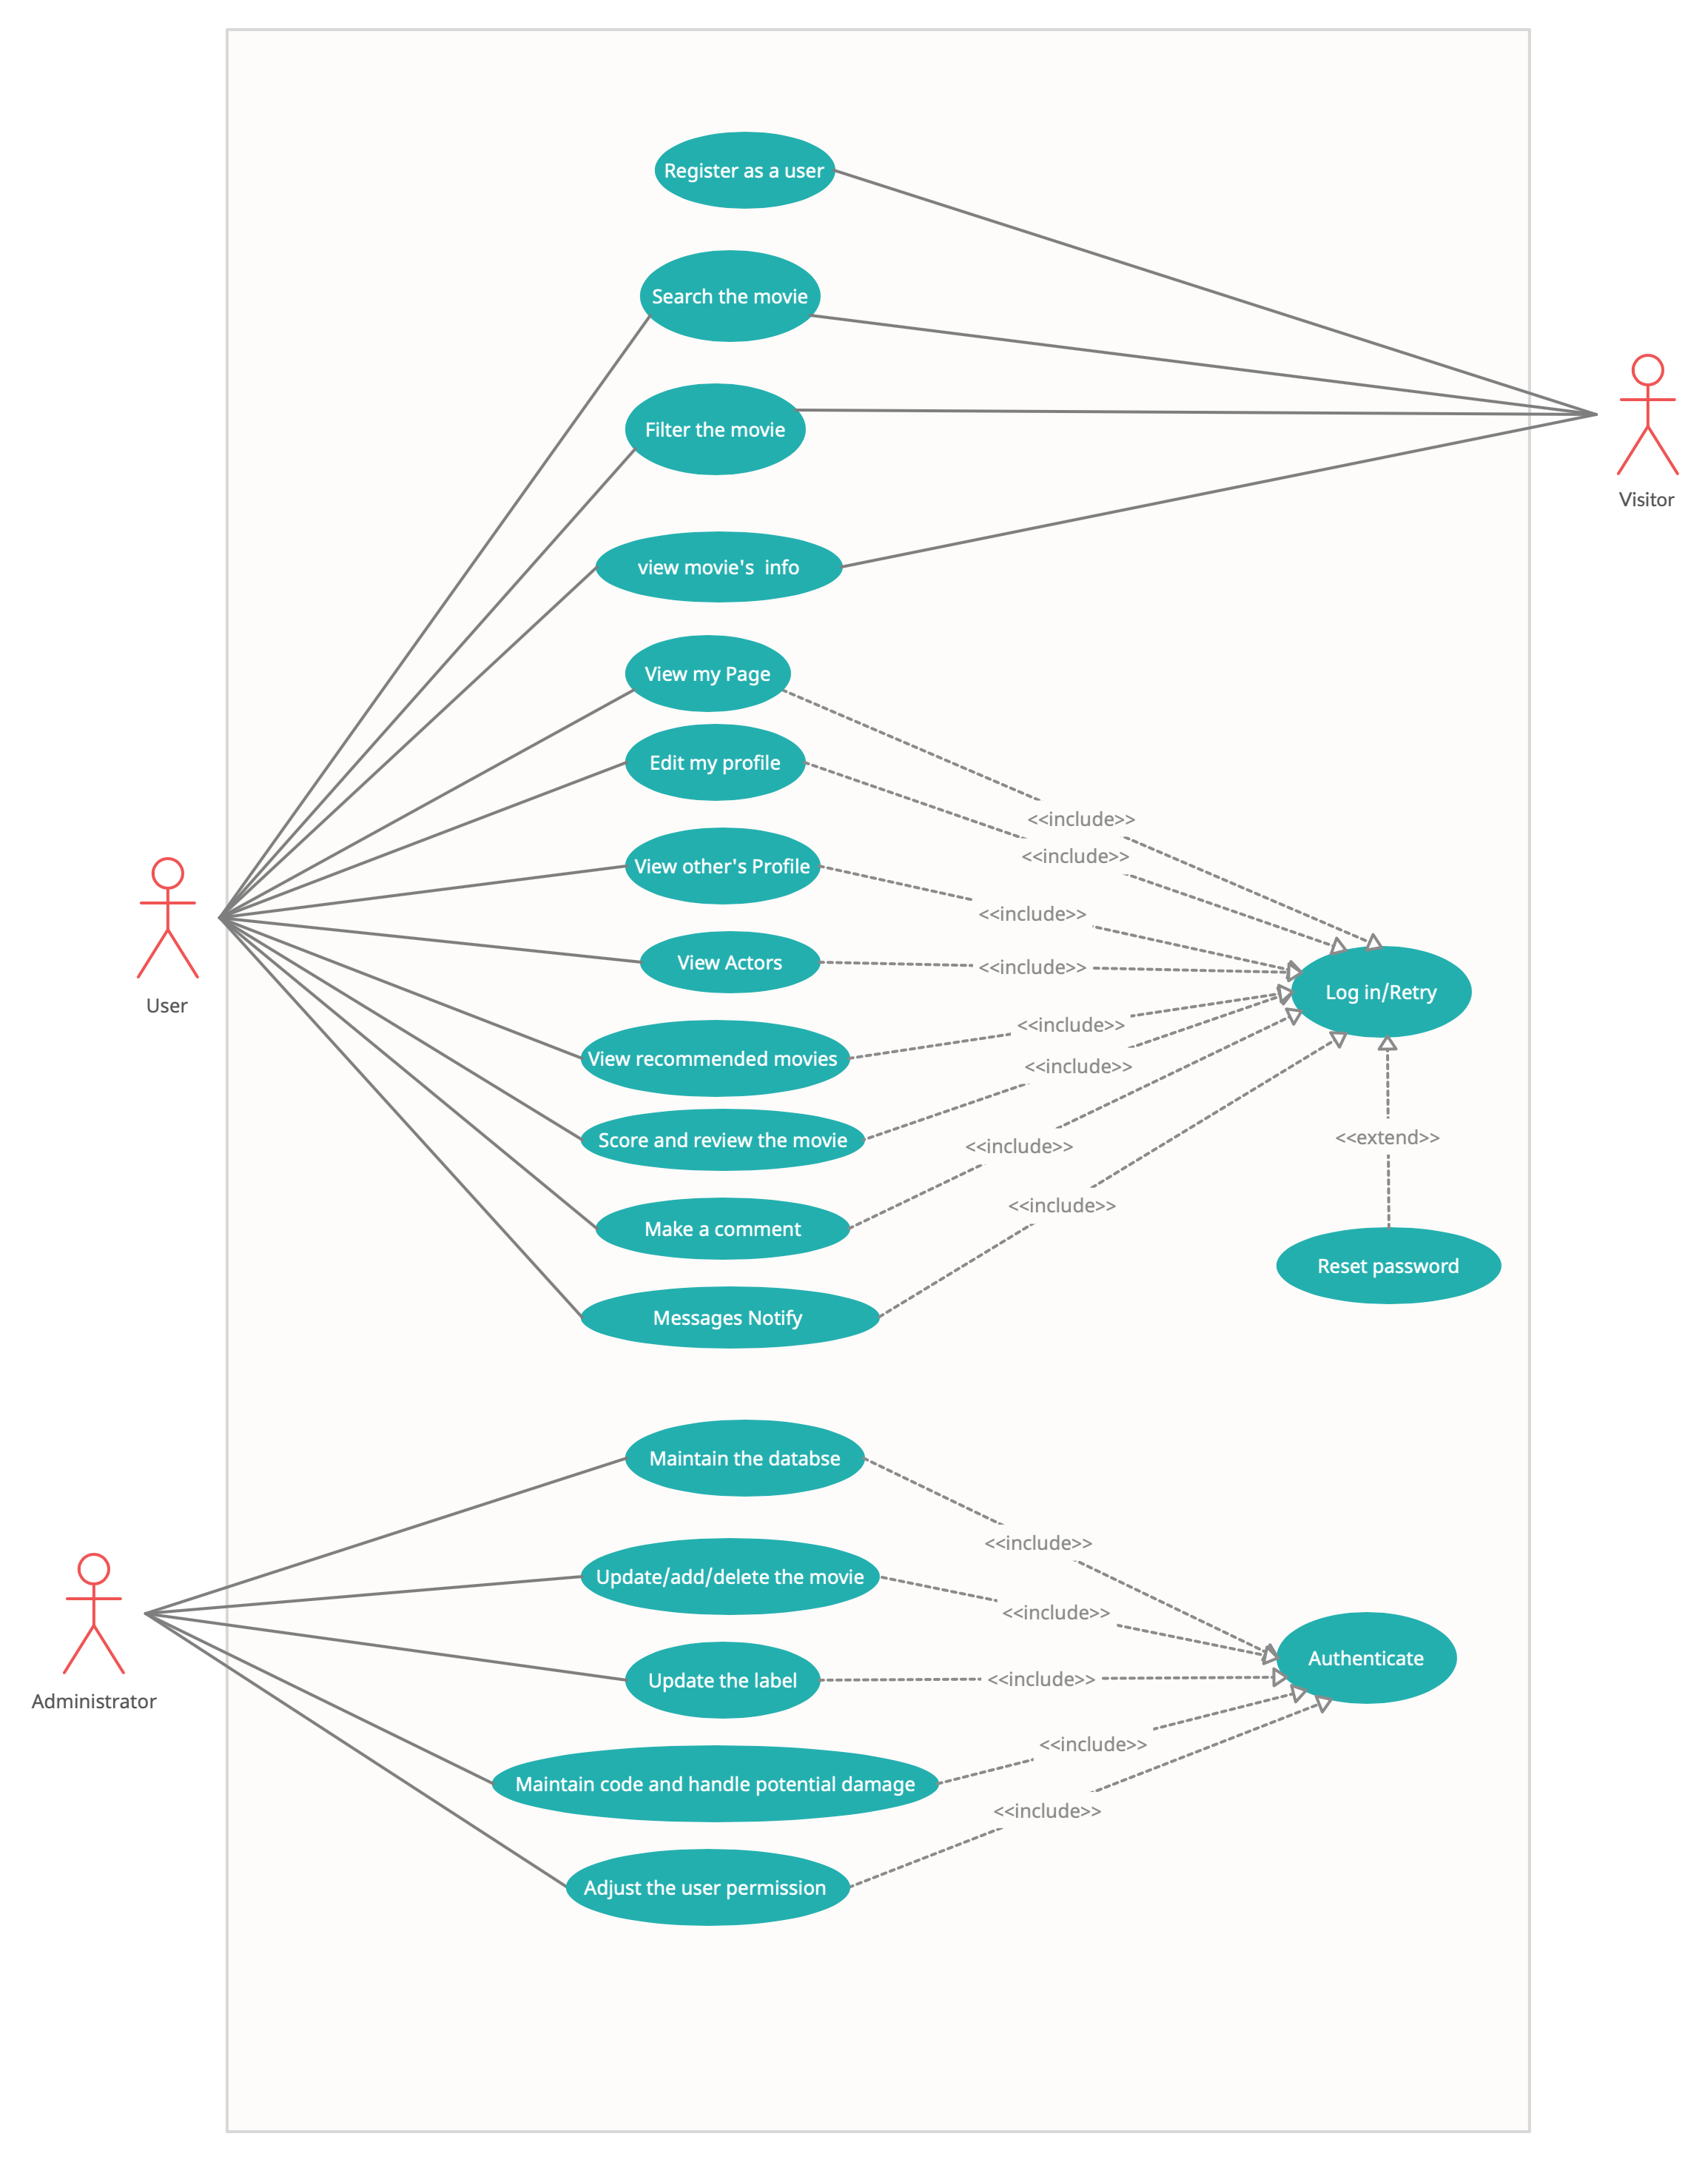
\includegraphics[width=1\linewidth]{UCD.png}\\\newpage
\subsection{Use Case Description}
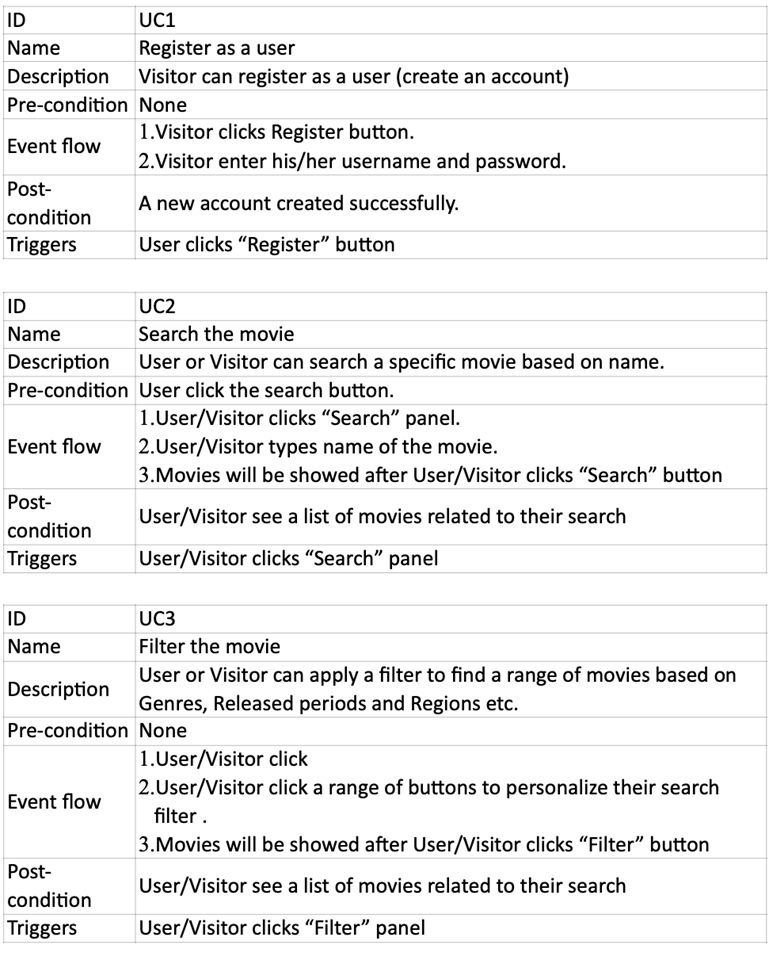
\includegraphics[width=1\linewidth]{UD1.png}\\
\newpage
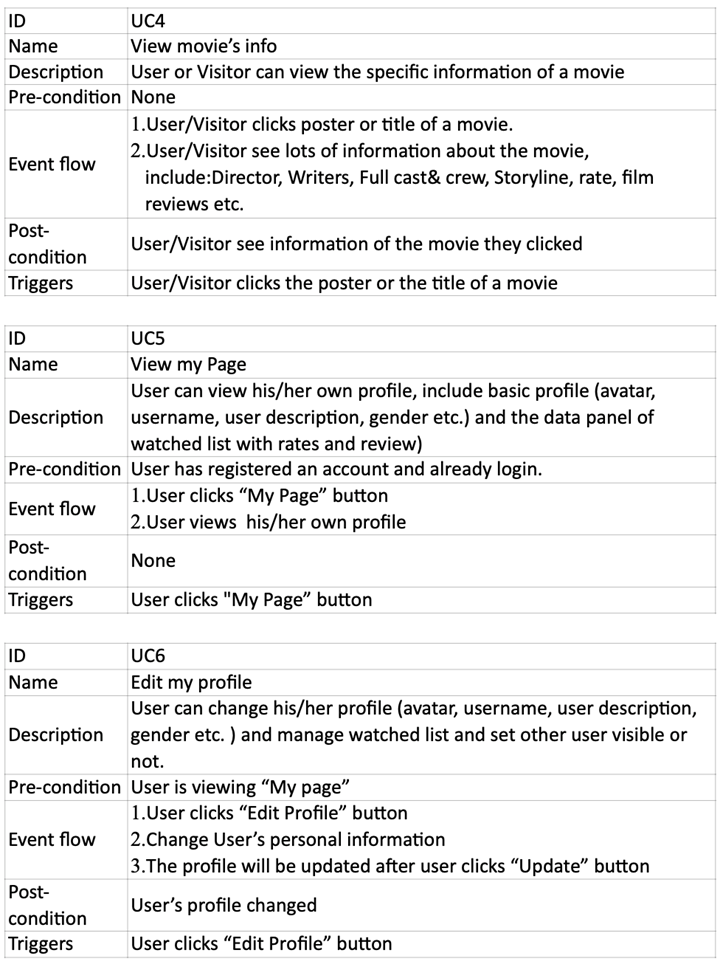
\includegraphics[width=1\linewidth]{UD2.png}\\\newpage
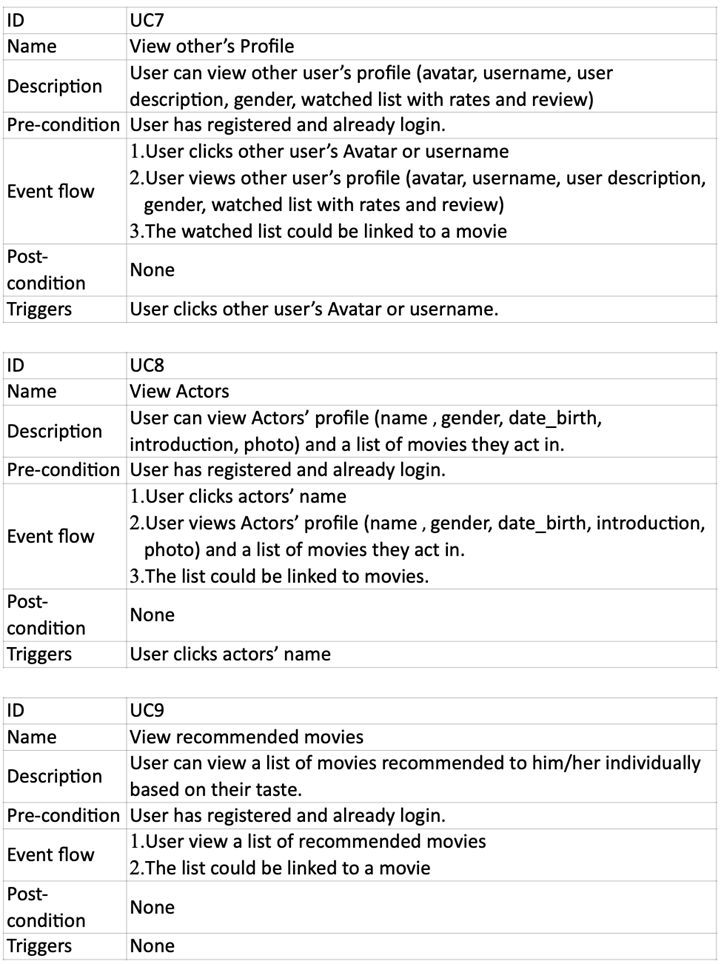
\includegraphics[width=1\linewidth]{UD3.png}\\\newpage
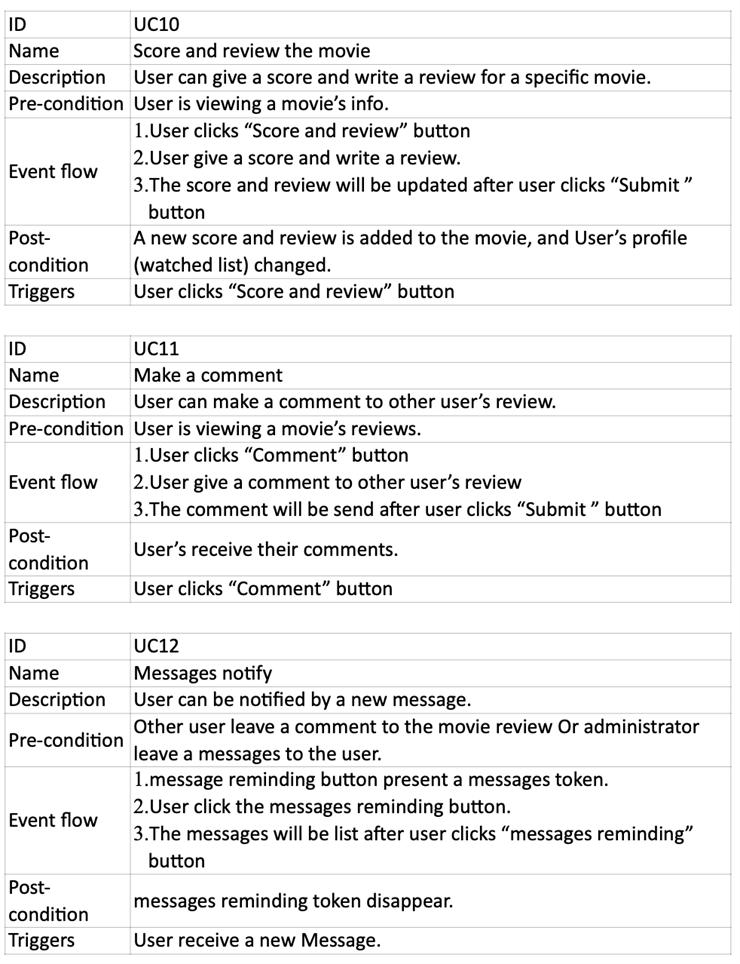
\includegraphics[width=1\linewidth]{UD4.png}\\\newpage
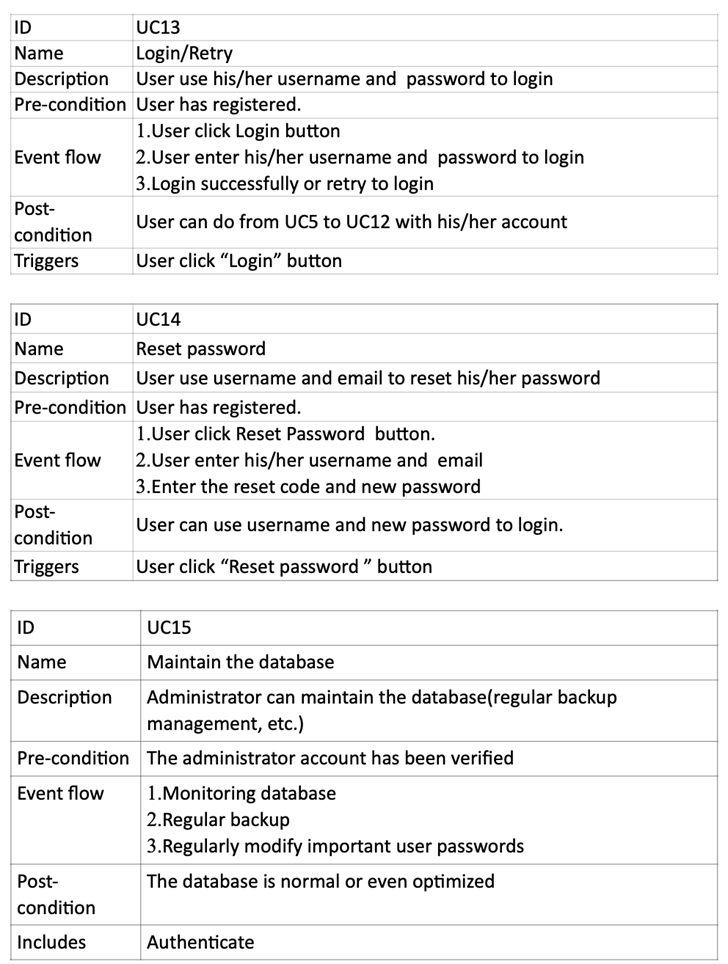
\includegraphics[width=1\linewidth]{UC4.png}\\\newpage
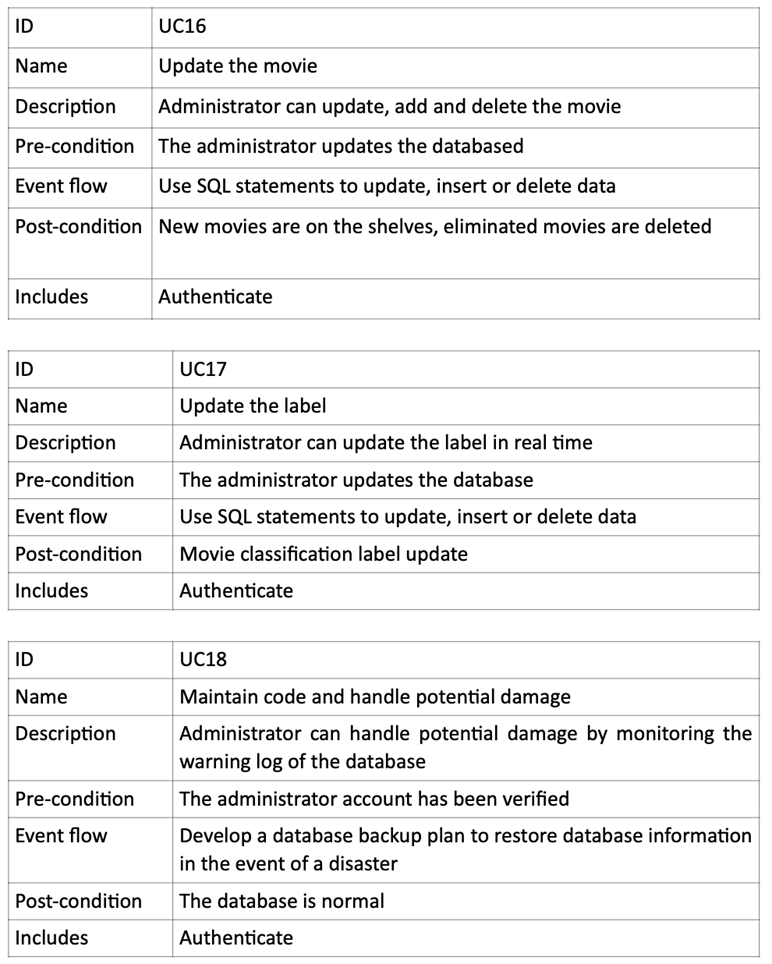
\includegraphics[width=1\linewidth]{UC5.png}\\\newpage
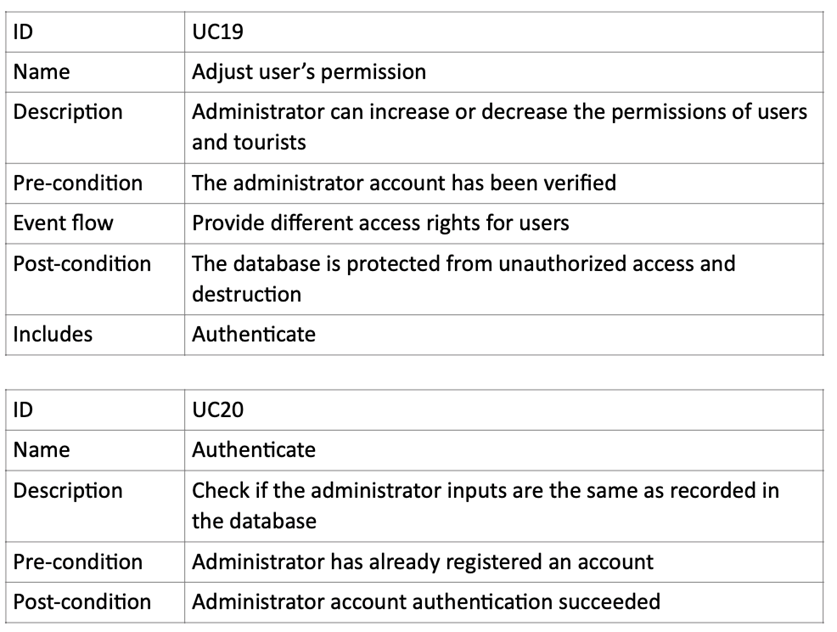
\includegraphics[width=1\linewidth]{UC6.png}\\\newpage
\subsection{Data Flow Diagram}
\vspace{1cm}
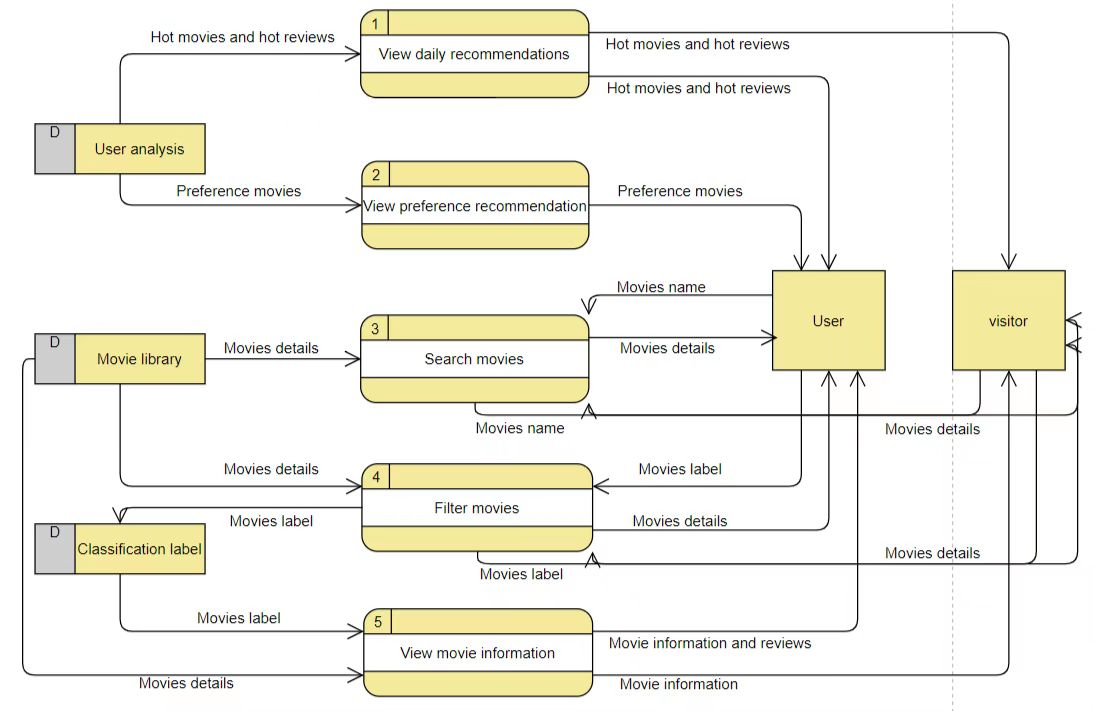
\includegraphics[width=1\linewidth]{DATA.jpg}\\\\\\
Data from the input of users and visitors flows to the movie's data repository and tag data repository through search and filtering. The repository feeds movie information back to users and visitors. The collaborative filtering algorithm flows the movie data that users may like to users, and flows popular movies to users and visitors.\\\newpage
\subsection{Navigation structure diagrams}
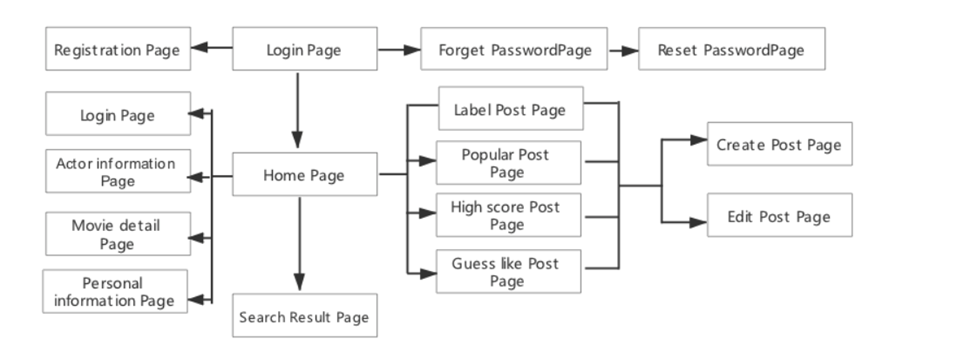
\includegraphics[width=1\linewidth]{nav.png}\\
In an actual HTML file, the header sections would be the same as the POST page, and they would serve as the navigation bar for the page. On the home page, users can choose to go to each of the four sections.Pages that have a search bar if the user.Enter the keyword in the search bar. In addition, there is a sidebar on the label page, popular page, high score page and guess sample page.The first is the regis-tration page, you can choose to register/login or directly enter the page, you can al-so go to the registration page, registration or directly login successfully can choose three parts of the page, the first is the home page, the second is the rank page, the third is the personal home page. A search on the home page for a key actor or a detailed movie will lead to two pages. The ranking page includes some key tabs for corresponding ranking, and also summaries the introduction of each movie. Per-sonal homepage includes personal information, history of movies watched. When you register, you need to use a valid email address and a password you set to log in successfully.\\

\subsection{Interface Design}
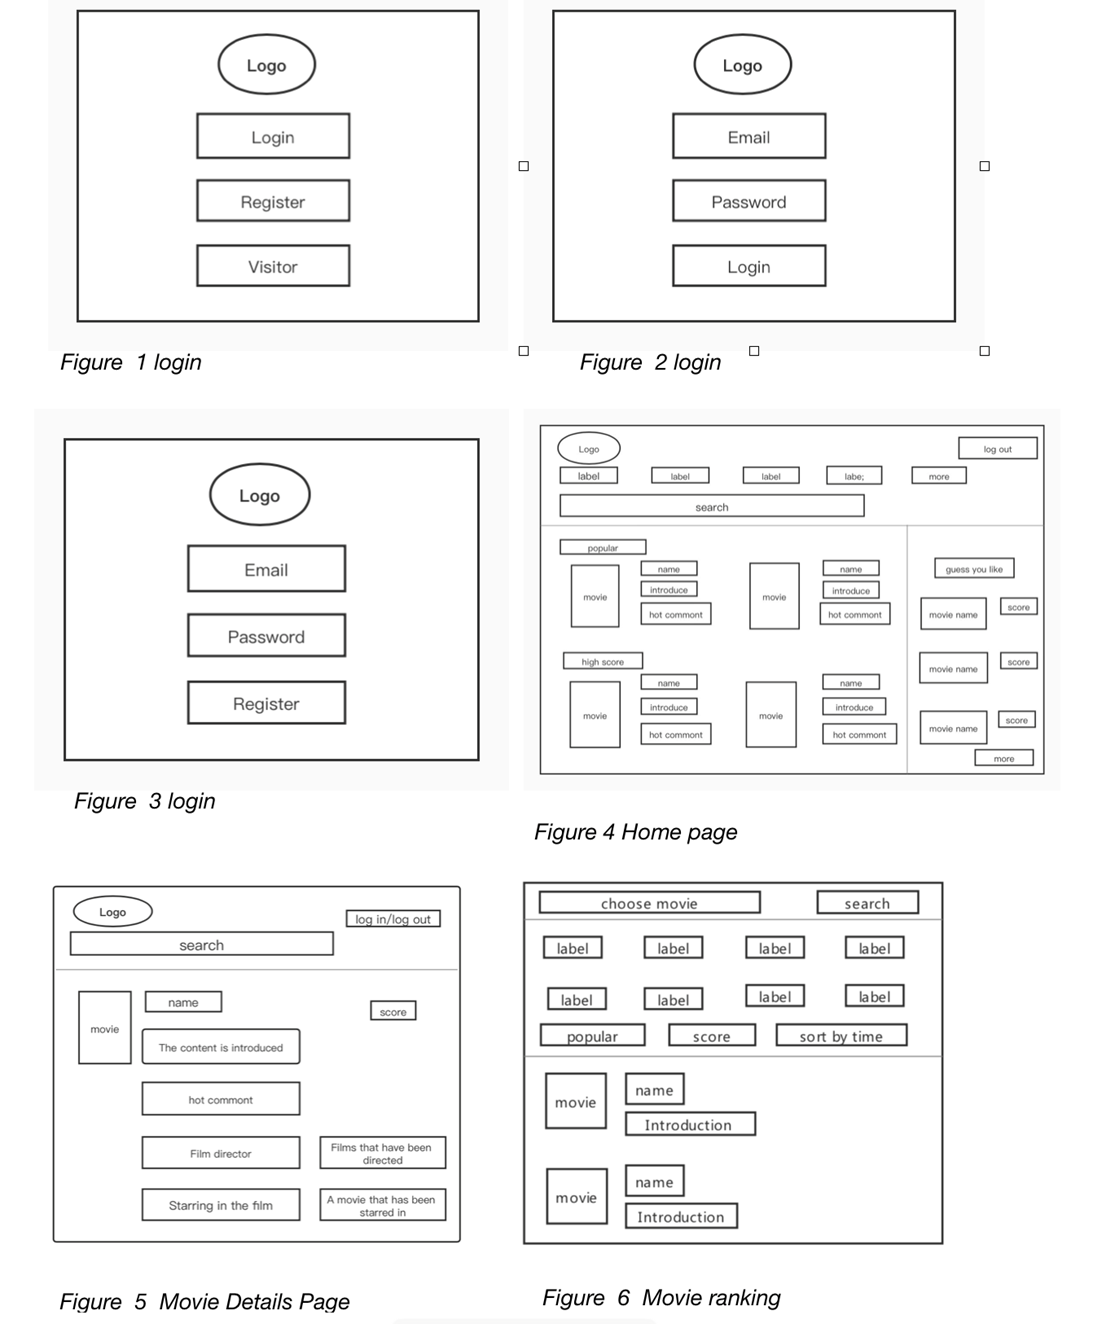
\includegraphics[width=1.1\linewidth]{inter.png}\\\newpage
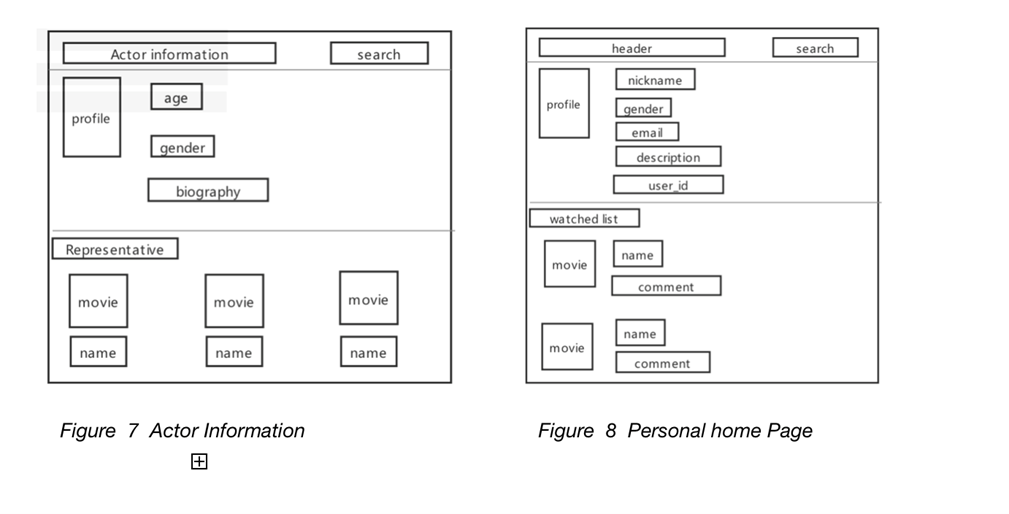
\includegraphics[width=1.1\linewidth]{int2.png}\\
\subsection{Story Board}
\includegraphics[width=1\linewidth]{Story.jpg}\\\newpage

\section{Testing Design}
\subsection{Testing Strategy}
Three phases of testing is required for testing stage: unit testing, integrated testing and system\&acceptance testing. A testing document will be used to record the bugs and errors found within the whole implementation stage. In addition, a test report will be delivered, which will include functional testing, performance testing and security testing.\\\\
unit testing will cover every individual unit of the system, on how they perform separate from each other. The strategy for the unit testing will be white-box testing. This will allow the testing members to check the code, input the test data and see exactly what’s going on and how it’s affecting the output. \\\\
Integration testing will test how the unit work together as a sub-system. Bottom-up testing is used in this phase. Testing members will test different aspects of sub-systems starting with the lower levels of the system. Integration testing is a key phase of testing since many bugs can be found and early release versions of the overall software or hardware can be developed.\\\\
System\&acceptance testing will test the whole system. The strategy for system\&acceptance testing is black-box testing. Testing team will give test data and cases based on the specification for functional testing and they will use WebPageTest to deliver performance testing and security testing report. Finally, once demo version of our project delivered, an acceptance and satisfaction survey will be made. The group will change settings and develop further functionality based on the survey.
\subsection{Test Form}
Testing team is aimed at finding bugs and defects within the system and to ensure that it matches the requirements of the project.\\
\begin{figure}[h]
    \centering
    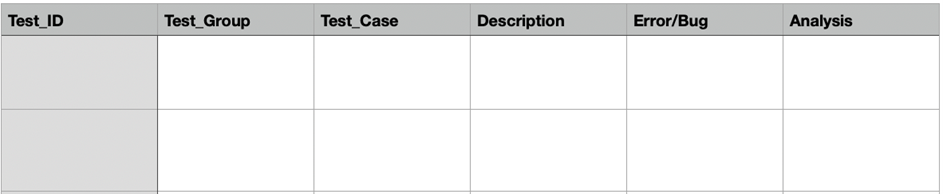
\includegraphics{tf1.png}
    \caption{Unit Testing form}
\end{figure}
\begin{figure}[h]
    \centering
    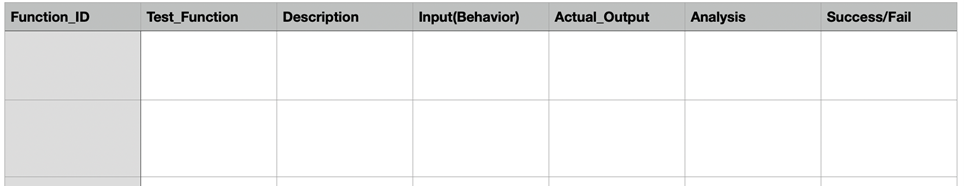
\includegraphics{tf2.png}
    \caption{Functional testing form}
\end{figure}
\\
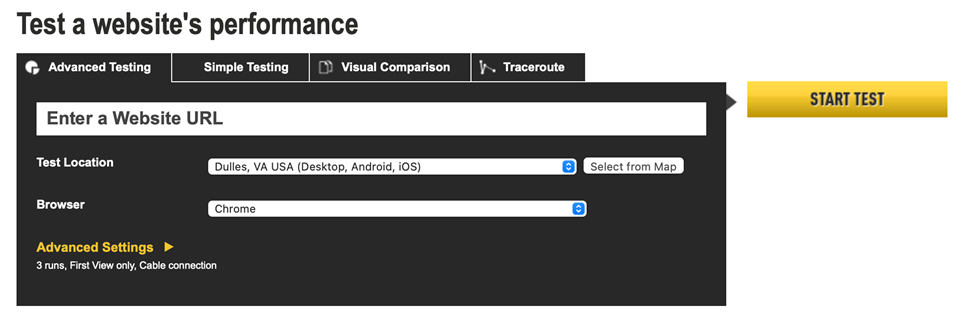
\includegraphics[width=1\linewidth]{tf3.png}{\\Performance testing and security testing WebPageTest: https://www.webpagetest.org}

\newpage
\section{Planning and Risk Assessment}
\subsection{Planning}
The basic idea for planning is that, every members could take part in different part of our Project,  the  multi-cross assignment make our project motivated and enhance the efficient communication between different groups.\\
We chose to be using Agile methodology for developing software. Agile development make our project has the advantages of adaptive planning, evolutionary development, early delivery, and continual improvement. \\
The task and code will be developed modularly, which means they are easy to manage and we can work on different task simultaneously.\\\\
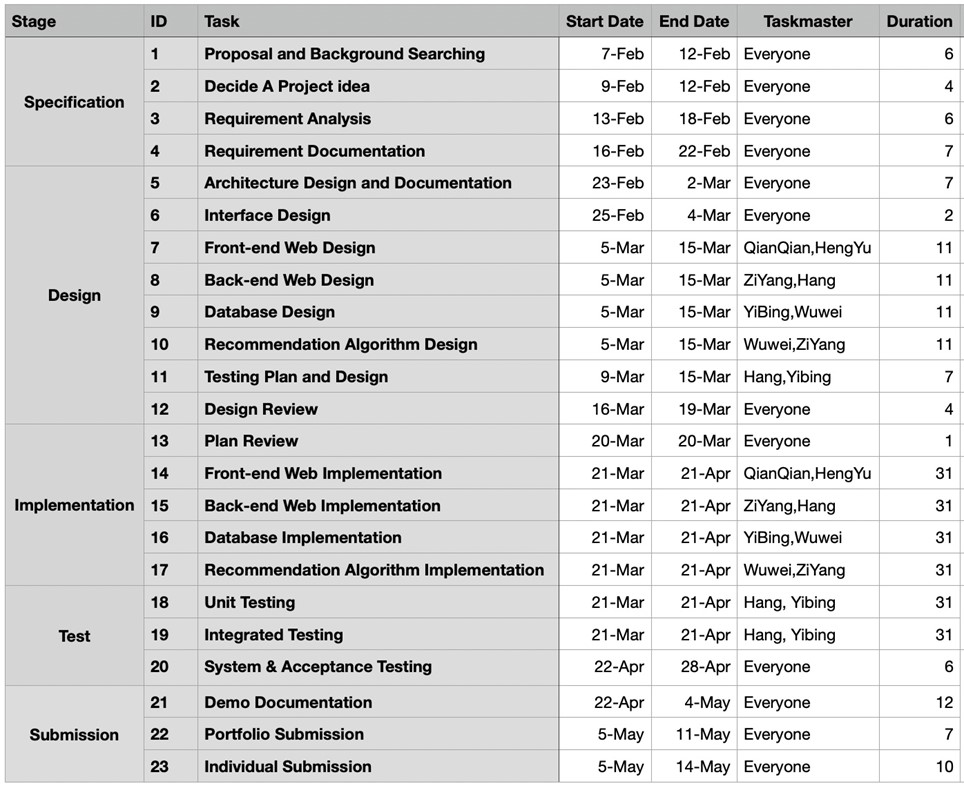
\includegraphics[width=1\linewidth]{PD.jpg}
\newpage
\subsection{Required Skills}
•	Git command and Github is considered as an important skill, which will improve the efficiency of coding as a group work. \\
•	PHP, JavaScript , MySQL for back-end implementation.
•	HTML, CSS for front-end Implementation.\\
•	Python is used to build recommendation algorithm (Item based Collaborative Filtering Algorithm etc.). \\
•	Except  White-box testing, black-box testing, WebPageTest will be used for Functional and performance testing.\\ 
•	Communication skill is required, especially for the communication between the back-end group and front-end group. \\
\subsection{Challenge}
\subsubsection{General Challenge} 
- Due to the pandemic virus, two of team members are outside the UK, so it could be a challenge for team members to host efficient communications online.\\
-Team members should learn related coding environment at the beginning of implementation, they also have to get to know how each part cooperation. \\
- Sets of new skill required, teams must learn and Implement over very short periods of time. \\
\\
\subsubsection{Technological Challenge} 
- For collaborative filtering algorithm,  as the number of users continues to increase, "nearest neighbor search" within a large number of users will become the bottleneck of the entire algorithm, and the amount of calculation is large.\\
-	It’s a challenge transfer XML data from TMDb data to  SQL format.\\
-	It’s hard for Front-end design to deliver a user-friendly interface.\\\newpage



\section {References}
\noindent [1] Hameed, M.A, O. Al Jadaan and S. Ramachandram, Collaborative filtering based recommendation system: A survey. International Journal on Computer Science and Engineering, 4(5), 859, 2012.\\
\\
\noindent [2] G. Author, "8 Major Advantages of Using MySQL", Datamation.com, 2016. [Online]. Available: https://www.datamation.com/storage/8-major-advantages-of-using-mysql.html. \\\\
\noindent [3] “The Movie Database (TMDb) API”, TMDb, 2021. [Online] Available:\\ https://developers.themoviedb.org//3/getting-started/introduction [Accessed: March-2021].\\\\
\noindent [4] “The Movie Dataset”, Kaggle, 2021. [Online] Available:\\ https://www.kaggle.com/rounakbanik/the-movies-dataset [Accessed: March-2021]\\\\
\noindent [5] “TMDB 5000 Movies Dataset”, Kaggle, 2021.[Online] Available:\\ https://www.kaggle.com/tmdb/tmdb-movie-metadata [Accessed: March-2021]\\

\end{document}
